\section{The Alma Dancer}

Woman is not a “thing”, but an animal, which is worse: she is becoming a marionette, since that is what man liked. The aversion for woman, with that sacred fixation of “value”, is a modern obsession that proves the weakness of European man as ascetic and as warrior. The two attitudes that man should adopt before woman are all there: pure attitudes not dulled by rancor or bitterness.

\begin{wrapfigure}{rt}{.3\textwidth}
 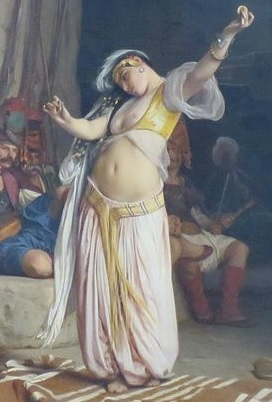
\includegraphics[scale=.5]{a20150517TheAlmaDancer-img001.jpg}
\caption{Alma Dancer}
\end{wrapfigure}

The Easterner, unlike a vulgar man, sees things differently: he knows that woman is a being whose superiority is obvious in a domain where man is very poor: freedom — although without light and without consciousness like children — an absence of prejudices, miraculous clarity, and a smile that man calls “evil”; not affirmation, but a shrug of the shoulder in the face of what man builds in a bourgeois way; to be capable of everything, accessible to everything, the receptacle of everything, bottomless, symbol of the cosmic matrix, insatiable. The Easterner, who is man in an absolute sense that the Westerner does not know, owes that to the fact that he is also woman, a thing that the Westerner will never know how to be.

That is why the Easterner is exquisite with woman; he caresses her, kills her, and confines her. He gives her, in short, her true freedom, her real strength. Taken such as she is, and not as man constructs her, woman has a value and that is why divinity gave her that miraculous thing which is the dance: the rhythm of her hip, the song the crowns the rhythm, the smile of evasion that is found only in the Ascetic who swims and empties himself: that smile that in maithuna [sexual union in Tantra] man does not have and only woman has, and who, speaking aesthetically, is visible only on certain Khemer heads. And I never saw the outcrop of the inexpressible change so well in plastic fixation except on those Khmer stones, and in the sculpture of Ellora, absolute figuration of absolute conjunction and absolute integration — beatitude, ananda.

That is the smile that woman, the sleeping child, and the Ascetic have: man attains this smile only when the infusion is absolute, when the sea overflows the rivers and waters. The Easterners see things thus, they can only see things thus.

At the time of medieval Chivalry, there was in man — this is mathematically certain — a freedom that he no longer has, and in woman, a submission and a sweetness that she can find again today only if man becomes again simple man, that is to say, more woman. Let Man be woman, and we will see what woman will become: a very fertile, docile, subtle being. At present the European is a Male and woman a Female wearing the mask of the Male. But man truly man (the East) more feminine than woman, subtle, ophidian, makes woman become again what she is.

Practically: let woman no longer roam about, let her be locked up, let her be respected; let what Westerners call “corruption” be, not exterior and visible, but confined — therefore free, not traditional. Women in the house and men outside: and you will see the action of woman — Dionysian, dissolving, Maenad-like action — recover her ancient strength.

In regard to the woman, the Islamic system was complete, whole. In Europe, the situation is horrendous: man pushes woman into the street, removes her veil, prostitutes her in sunlight, places her where she cannot be, where it is against nature for her to be: in the schools, trains, cafes, in the pigsty. The Anglo-Saxon peoples wanted that: and among us, with the stupidity that pushes us toward the ordure, we are following the example of those coarse beasts.

One final observation: the dance is solo (Oriental dance: the belly dance): Europe destroyed that, too, and introduced the couple's dance. If we follow the thread of this thought, we will go very far in the vision of Western perversion.


\hfill

\textbf{Guido De Giorgio}'s essay \textit{Short Notes on Ascesis and Anti-Europe}\footnote{\url{https://www.gornahoor.net/?p=6397}} is missing a note. Although this section was present in the original Ur journal and even the first collections, it was excluded in all the editions after 1955. I don't know why.

This note is collected in \textit{L'Instant et l'Eternité}. It appeared just before the incident about the sirocco in Tunisia. It extols the Traditional role of woman, particularly as it was, and might still be, found in Islamic nations.



\flrightit{Posted on 2013-05-17 by Cologero }

\begin{center}* * *\end{center}

\begin{footnotesize}\begin{sffamily}



\texttt{Saladin on 2013-05-21 at 22:46 said: }

while agreeing with De Giorgio's tenants and his overall Weltanschauung, I understand why these paragraphs were omitted. They are totally confusing (at least to me).


\hfill

\texttt{Cologero on 2013-05-21 at 23:25 said: }

Saladin, is the incomprehension the fault of the translation? If any passages are unclear, I can take another try at them.


\hfill

\texttt{Saladin on 2013-05-23 at 19:51 said: }

I doubt it is due to translation (and let me thank you once more for all the precious translations you have made available). In my humble opinion the passages do not completely make sense.

Take for example this paragraph: “The Easterner sees things differently: he knows that woman is, opposite vulgar man, a being whose superiority is obvious in a domain where man is very poor: freedom—although without light and without consciousness like children—an absence of prejudices, miraculous clarity, and a smile that man calls “evil”.

What does De Giorgio really wants to convey? That woman is more liberated (in spiritual sense) and less prejudiced? Cologero, I am sure you have a better grasp of what De Giorgio wants to convey here. Maybe you can clarify and comment on these passages which will be very much appreciated.

I really enjoyed your other translations of De Giorgio and I can only think that he himself decided that above note was not entirely coherent and he decided to omit from subsequent editions.

What does he really mean when he say: “Let Man be woman, and we will see what woman will become: a very fertile, docile, subtle being.”?


\hfill

\texttt{Mihai on 2013-05-24 at 03:42 said: }

I have read somewhere a comment by Evola in which he describes DeGiorgio as a “chaotic type of initiate”. I really wondered what he meant by that, but now, like you, I know.

\hfill

\texttt{Saladin on 2013-05-24 at 19:15 said: }

I had read that same comment (I am pretty sure on this blog) by Evola but totally forgotten it. However, granted De Giorgio may not be as lucid as Evola but I think he is nevertheless Traditional and immensely interesting.


\end{sffamily}\end{footnotesize}
